\chapter{Ferramentas \Hets e \Isabelle}
\label{chap:hetseisabelle}

Ambas as ferramentas \Hets e \Isabelle possuem integração com o editor de texto \textit{emacs}.
Através dessa integração, pode-se escrever as especificações com coloração de sintaxe no editor e, então, utilizar as duas ferramentas para efetuar análise sintática e escrever provas.
Neste capítulo, descreve-se sucintamente o uso de cada uma das ferramentas.

\section{Verificando especificações com \Hets}
A ferramenta \Hets pode ser invocada dentro do editor de texto \textit{emacs} de duas formas: na primeira, ela apenas realiza a análise sintática da especificação contida na janela atual; na segunda forma, após realizar a análise sintática, o grafo de desenvolvimento é gerado, mostrando a estrutura da especificação analisada. Para a especificação da biblioteca deste trabalho, o grafo resultante pode ser visto na \citeFig{fig:ProofStart}.

\begin{figure}[hp]
	\centering
		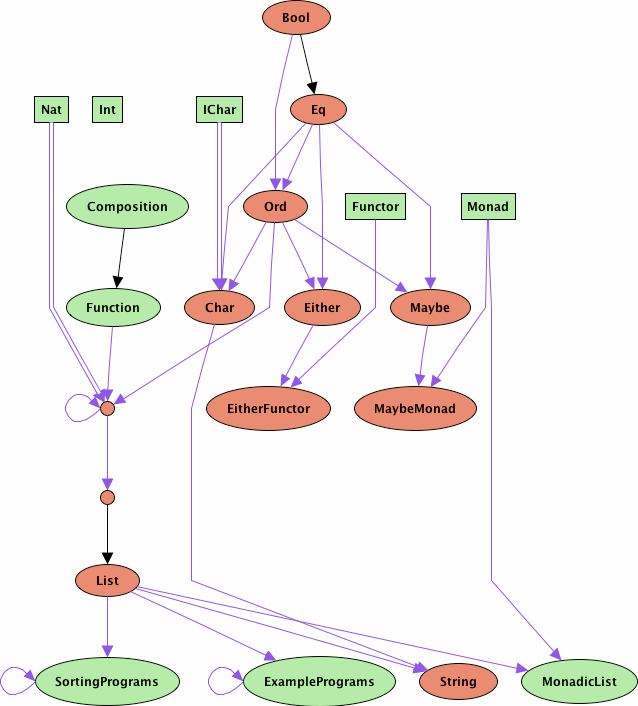
\includegraphics[scale=0.7]{"figuras/ProofStart.png"}
	\caption{Estado inicial das provas da biblioteca na ferramenta Hets}
	\label{fig:ProofStart}
\end{figure}

Na figura, os nós elípticos representam uma especificação do arquivo que foi analisado.
Os círculos indicam subespecificações, ou seja, trechos de especificações que foram separados pela declaração \Verb.then..
Os retângulos indicam especificações importadas de outras bibliotecas.
No caso deste trabalho, todas foram importadas da biblioteca da linguagem \CASL.
Os nós vermelhos (cinza escuro) indicam especificações que possuem um ou mais teoremas a serem provados.
Os nós verdes (cinza claro) não possuem teoremas ou todos os seus teoremas já estão provados.

A partir do grafo pode-se iniciar o provador de teoremas \Isabelle para verificar os teoremas existentes nos nós. Uma prova típica se inicia pelo método automático de prova sobre a estrutura da especificação. Este método analisa as teorias presentes e as diretivas (\Verb.%mono., \Verb.%implies., etc.), construindo as dependências entre as especificações e revelando os nós ocultos das subespecificações que contêm teoremas a serem provados.

O próximo passo é utilizar o provador \Isabelle para verificar os teoremas existentes nos nós vermelhos. Para tanto, basta escolher um nó e, com o botão direito, escolher a opção \textit{Prove}. A janela seguinte permite escolher um entre vários provadores de teoremas. Para a linguagem \HasCASL, o provador \Isabelle precisa ser usado. Esta opção irá efetuar a tradução da especificação para uma teoria correspondente em \HOL, exibindo a mesma em uma outra janela do editor \textit{emacs}, permitindo com que a prova dos teoremas seja escrita.

Após processar todo o arquivo de provas, pode-se fechar o editor de texto e o estado desta prova será atualizado no grafo. Se a prova foi finalizada com sucesso, o nó correspondente terá sua cor alterada para verde. Caso contrário, sua cor permanecerá vermelha. Quando todos os nós circulares correspondentes a subespecificações de um nó elíptico tiverem a cor alterada para verde, eles novamente se tornarão ocultos, e apenas o nó elíptico correspondente à especificação completa será exibido.

Algumas provas de teoremas da especificação da biblioteca ainda permanecem em aberto, como ilustram os nós vermelhos da \citeFig{fig:ProofEnd}. A maior parte das provas em aberto estão relacionadas à falta de suporte de construtores de classes na linguagem \HOL. Métodos alternativos de tradução para \Isabelle/\HOL estão em investigação pelo grupo responsável pela ferramenta \Hets.

\begin{figure}[hp]
	\centering
		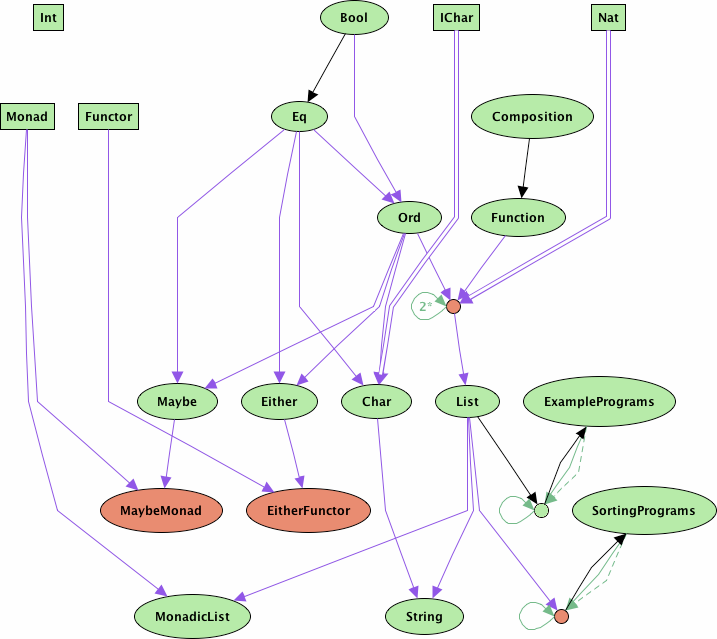
\includegraphics[scale=0.6]{figuras/ProofEnd.png}
	\caption{Estado atual das provas da biblioteca na ferramenta Hets}
	\label{fig:ProofEnd}
\end{figure}

\section{Usando o provador de teoremas \Isabelle}
A tarefa de verificar os teoremas gerados pela especificação, embora não fosse o foco do trabalho, tornou-se a parte mais complexa. Embora ainda permaneçam teoremas em aberto, a maioria pode ser verificado. A seguir, explica-se como se deu o processo de construção das provas.

A maior parte das provas foi iniciada pelo comando \Verb.apply(auto). porque desejava-se que \Isabelle agisse de forma automática, sempre que possível. Abaixo, ilustra-se a prova de um teorema da especificação \Verb.Bool.:

\begin{Verbatim}
theorem NotFalse1 : "ALL x.
 Not' x = True' = (x = False')"
apply(auto)
apply(case_tac x)
apply(auto)
done
\end{Verbatim}

A seguir, os comandos da prova são explicados:
\begin{itemize}
\item \textit{apply (auto)}:

Este comando simplifica a proposição atual de forma automática, indo o mais longe que conseguir nas reduções.
Neste teorema, o comando apenas conseguiu eliminar o quantificador universal, produzindo o resultado a seguir:

\begin{Verbatim}
goal (1 subgoal):
 1. !!x. Not' x = True' ==> x = False'
\end{Verbatim}

\item \textit{apply (case\_tac x)}:

O método \textit{case\_tac} atribui uma valoração possível para a variável \Verb.x., substituindo-a por cada um dos construtores do tipo a que a variável pertence.
Aqui, como a variável \Verb.x. é do tipo \Verb.Bool., \Verb.x. foi instanciado para os construtores \Verb.True. e \Verb.False.:

\begin{Verbatim}
goal (2 subgoals):
 1. !!x. [| Not' x = True'; x = False' |] ==> x = False'
 2. !!x. [| Not' x = True'; x = True' |] ==> x = False'
\end{Verbatim}

\item \textit{apply (auto)}:

Desta vez, o comando automático foi capaz de terminar a prova automaticamente.

\begin{Verbatim}
goal:
No subgoals!
\end{Verbatim}

\end{itemize}

Um exemplo de prova para um teorema da especificação \Verb.Eq. é mostrado a seguir.
Nesta prova, foi introduzido o comando \Verb.simp add:., que espera uma lista de axiomas ou teoremas previamente provados como parâmetros para serem utilizados em uma tentativa automática de simplificar a proposição corrente.
Este comando faz uso, além dos teoremas passados como parâmetro, dos demais axiomas no escopo da teoria atual.
Se a proposição não pode ser reduzida, o comando produz um erro; caso contrário, uma nova proposição é gerada, caso a prova não tenha sido concluída automaticamente.

\begin{Verbatim}
theorem DiffTDef :
"ALL x. ALL y. x /= y = True' 
= (Not' (x ==' y) = True')"
apply(auto)
apply(simp add: DiffDef)
apply(case_tac "x ==' y")
apply(auto)
apply(simp add: DiffDef)
done
\end{Verbatim}

Os teoremas usados na prova anterior também foram utilizados em várias provas da especificação \Verb.Ord..
A prova do teorema \Verb.%(LeTAssimetry)%. destaca-se das demais por introduzir a necessidade de criar lemas auxiliares.
Em alguns casos, um axioma ou teorema precisa ser reescrito de forma que o \Isabelle consiga utilizá-lo em suas provas automáticas.
Para tanto, cria-se um lema, que apesar do nome, funciona da mesma forma que um teorema.
No caso do teorema \Verb.%(LeTAssimetry)%., utilizou-se o comando \Verb.rule ccontr. para iniciar uma prova por contradição.
Após algumas simplificações, o provador \Isabelle não foi capaz de utilizar o axioma \Verb.%(LeIrreflexivity)%. para simplificar o objetivo e produziu:

\begin{Verbatim}
goal (1 subgoal):
 1. !!x y. [| x <' y = True'; y <' x = True' |] ==> False
\end{Verbatim}

Foi necessário criar o lema auxiliar \Verb.LeIrreflContra., provado automaticamente pelo provador \Isabelle.
O teorema foi interpretado internamente da seguinte forma:

\begin{Verbatim}
?x <' ?x = True' ==> False
\end{Verbatim}

Pode-se, então, induzir a ferramenta \Isabelle a usar o lema anterior forçando a atribuição do valor \Verb.x. para a variável \Verb.?x. através do comando \Verb.rule_tac x="x" in LeIrreflContra..
A mesma tática foi utilizada para forçar o uso do axioma \Verb.%(LeTTransitive)%..
A prova foi finalizada com o comando \Verb.by auto..

\begin{Verbatim}
lemma LeIrreflContra :
  " x <' x = True' ==> False"
by auto

theorem LeTAsymmetry :
"ALL x. ALL y. x <' y = True'
  --> y <' x = False'"
apply(auto)
apply(rule ccontr)
apply(simp add: notNot2 NotTrue1)
apply(rule_tac x="x" in LeIrreflContra)
apply(rule_tac y="y" in LeTTransitive)
by auto
\end{Verbatim}

Alguns usos do comando \Verb.apply(auto). podem entrar em laços infinitos.
Um exemplo ocorreu quando os teoremas das especificações \Verb.Maybe. e \Verb.Either. foram provados.
Para evitar o laço infinito, a regra de eliminação do quantificador universal foi aplicada diretamente, usando o comando \Verb.apply(rule allI)..
O comando \Verb.rule. aplica o teorema ou axioma especificado diretamente, sem usar outras regras na redução.
Para remover mais de um quantificador, pode-se incluir o sinal \Verb.+. após a regra, indicando que a mesma deve ser utilizada repetidamente, até que não seja possível nenhuma outra simplificação.

Após remover os quantificadores, o comando \Verb.simp only:. foi aplicado.
Este comando, ao contrário do comando \Verb.simp add:., utiliza apenas as regras passadas como parâmetros para tentar simplificar o objetivo atual.
Na maior parte das vezes, os dois comandos podem ser usados sem distinção.
Algumas vezes, no entanto, o comando \Verb.simp add:. pode entrar em laços infinitos; nestes casos, o comando \Verb.simp only:. deve ser usado para que a simplificação seja possível.
Abaixo, mostra-se um teorema e sua respectiva prova para exemplificar o procedimento descrito.

\begin{Verbatim}
theorem IMO03 : "ALL x. Nothing >=' Just(x) = False'"
apply(rule allI)
apply(simp only: GeqDef)
apply(simp only: GeDef OrDef)
apply(case_tac "Just(x) <' Nothing")
apply(auto)
done
\end{Verbatim}

A especificação \Verb.ListNoNumbers. possui apenas o teorema \Verb.FoldlDecomp. em aberto.
Já a especificação \Verb.ListWithNumbers., que possui quatro teoremas, tem todos os seus teoremas em aberto.
No primeiro caso, quase todos os teoremas necessitaram de comandos de indução para serem provados.
\Isabelle executa indução sobre uma variável através do comando \Verb.induct_tac..
Este comando espera como parâmetro uma variável ou uma expressão sobre a qual deve executar o processo de indução.
A seguir, é apresentado um exemplo envolvendo indução oriundo da especificação \Verb.ListNoNumbers..

\begin{Verbatim}
theorem FilterProm :
"ALL f. ALL p. ALL xs.
 X_filter p (X_map f xs) = 
   X_map f (X_filter 
     (X__o__X (p, f)) xs)"
apply(auto)
apply(induct_tac xs)
apply(auto)
apply(case_tac "p(f a)")
apply(auto)
apply(simp add: MapCons)
apply(simp add: FilterConsT)
apply(simp add: MapCons)
apply(simp add: FilterConsT)
done
\end{Verbatim}

As especificações \Verb.Char. e \Verb.String. usam combinações de comandos apresentados nos exemplos acima e, dessa forma, não são exemplificadas aqui.

As provas da especificação do exemplo \Verb.ExamplePrograms. embora longas, usaram apenas três comandos, basicamente: \Verb.simp only:., \Verb.case_tac., e \Verb.simp add:..
Como o comando \Verb.simp add:. consegue, geralmente, simplificações maiores, optou-se por tentar usá-lo sempre que possível.
Nos casos em que o comando entrou em laços infinitos, ele foi trocado pelo comando \Verb.simp only:..
Um teorema nesta especificação ainda permanece em aberto.
A seguir, a prova do teorema \Verb.Program02. é mostrada como exemplo.

\begin{Verbatim}
theorem Program02 :
"quickSort(X_Cons True' (X_Cons False' Nil')) =
 X_Cons False' (X_Cons True' Nil')"
apply(simp only: QuickSortCons)
apply(case_tac "(%y. y <' True') False'")
apply(simp only: FilterNil FilterConsT FilterConsF)
apply(simp only: QuickSortNil)
apply(simp only: XPlusXPlusNil)
apply(simp only: XPlusXPlusCons)
apply(simp only: XPlusXPlusNil)
apply(case_tac "(%y. y >=' True') False'")
apply(simp only: FilterNil FilterConsT FilterConsF)
apply(simp only: QuickSortNil)
apply(simp add: LeFGeTEqTRel)
apply(simp only: FilterNil FilterConsT FilterConsF)
apply(simp only: QuickSortCons)
apply(simp only: FilterNil FilterConsT FilterConsF)
apply(simp only: QuickSortNil)
apply(simp only: XPlusXPlusNil)
apply(simp only: XPlusXPlusCons)
apply(simp only: XPlusXPlusNil)
apply(simp only: IBO5)
apply(simp only: FilterNil FilterConsT FilterConsF)
apply(simp only: QuickSortCons)
apply(simp only: FilterNil FilterConsT FilterConsF)
apply(simp only: QuickSortNil)
apply(simp only: XPlusXPlusNil)
apply(simp only: XPlusXPlusCons)
apply(simp only: XPlusXPlusNil)
apply(case_tac "(%y. y >=' True') False'")
apply(simp only: FilterNil FilterConsT FilterConsF)
apply(simp only: QuickSortNil)
apply(simp only: XPlusXPlusCons)
apply(simp only: XPlusXPlusNil)
apply(simp only: FilterNil FilterConsT FilterConsF)
apply(simp only: QuickSortCons)
apply(simp only: FilterNil FilterConsT FilterConsF)
apply(simp only: QuickSortNil)
apply(simp only: XPlusXPlusNil)
apply(simp only: XPlusXPlusCons)
apply(simp only: XPlusXPlusNil)
apply(simp add: LeFGeTEqTRel)
done
\end{Verbatim}

Todos os teoremas da especificação \Verb.SortingPrograms. ainda não tiveram suas provas finalizadas.
Embora, para todos eles, várias proposições intermediárias tenham sido provadas, o caso geral ainda permanece em aberto.
Para mostrar o progresso feito nas provas, um exemplo com alguns comentários é apresentado a seguir.
O comando \Verb.prefer. é utilizado para escolher qual proposição se quer provar ao se utilizar o provador \Isabelle no modo interativo.
O comando \Verb.oops. indica ao provador para desistir da prova e seguir em frente no arquivo de provas.

\begin{Verbatim}
theorem Theorem07 : "ALL xs. isOrdered(insertionSort(xs))"
apply(auto)
apply(case_tac xs)
(* Proof for xs=Nil *)
prefer 2
apply(simp only: InsertionSort)
apply(simp add: GenSortF)
(* Proof for general case *)
apply(simp only: InsertionSort)
apply(case_tac List)
apply(auto)
apply(case_tac "X_splitInsertionSort (X_Cons a (X_Cons aa Lista))")
(* Proof for xs= Cons a Nil *)
prefer 2
apply(simp add: GenSortF)
(* Proof for xs=Cons a as*)
apply(case_tac Lista)
apply(auto)
prefer 2
(* Proof for xs = Cons a (Cons b Nil)*)
oops
\end{Verbatim}
